\documentclass{article}
\usepackage[spanish]{babel}
\usepackage[numbers,sort&compress]{natbib}
\usepackage{graphicx}
\usepackage{url}
\usepackage{amsmath}
\usepackage{hyperref}
\usepackage{float}
\usepackage{color}
\definecolor{gray86}{gray}{.86}
\definecolor{gray75}{gray}{.75}
\definecolor{gray45}{gray}{.45}
\usepackage{listings}
\lstset{ 
language=C,                
basicstyle=\footnotesize,      
numbers=left,                  
numberstyle=\footnotesize,     
stepnumber=1,                   
numbersep=5pt,                  
backgroundcolor=\color{gray86},  
showspaces=false,              
showstringspaces=false,         
showtabs=false,                
frame=single,           
tabsize=2,          
captionpos=b,          
breaklines=true,        
breakatwhitespace=false,   
escapeinside={\%*}{*)}          
}
\usepackage{subfigure} 
\usepackage[top=15mm, bottom=15mm, left=15mm, right=15mm]{geometry}
\setlength{\parskip}{2mm}
\setlength{\parindent}{0pt}

\author{Abraham Azael Morales Juárez  1422745}
\title{Sistema multiagente}
\date{\today}

\begin{document}

\maketitle

\section{Introducción}
Este es un sistema donde hay un conjunto de entidades, que interaccionan entre sí, con estados internos propios pero que son capaces de reaccionar y cambiar según cambien sus vecinos. Se manejan 3 estados internos, un modelo conocido como SIR, susceptibles, infectados y recuperados \cite{REF1}. 
\section{Objetivos}
Al momento de crear a los agentes, hacer que algunos de ellos ya se encuentren vacunados contra la enfermedad y que desde el inicio formen parte del estado R.\\
Obervar el efecto ocasionado por agregar individuos vacunados desde el inicio del análisis de la epidémia.
\section{Resultados}
Los parámetros y un fragmento del código \citep{REF1} modificado y usado en la práctica están a continuación.  Se observó la influencia en la cantidad de individuos (agentes) infectados y la correlación de individuos ya vacunados y que por ende ya no podrían contagiar la enfermedad, debido a que para que exista un contagio se necesita estar dentro de un rango de cercanía de otro agente previamente infectado. 

\begin{lstlisting}[frame=single]
l <- 1.5
n <- 150               #Cantidad de agentes
pi <- 0.8              #Probabilidad de infeccion
pr <- 0.02             #Probabilidad recuperarse
v <- l / 30            #Velocidad del agente
pv <- seq(0,1,0.1)     #Probabilidad de vacunacion y formar parte de R
r <- 0.1 
agentes <- data.frame(x = double(), y = double(), dx = double(), dy = double(), 
estado  = character())
for (i in 1:n) {
  e <- "S"
  if (runif(1) <= pi) {
    e <- "I"
    if (runif(1) <= pv) {
      e <- "R"
    }
  }
  agentes <- rbind(agentes, data.frame(x = runif(1, 0, l), y = runif(1, 0, l),
                                       dx = runif(1, -v, v), dy = runif(1, -v, v),
                                       estado = e))
  levels(agentes$estado) <- c("S", "I", "R")
}
   \end{lstlisting}

Estos agentes vacunados se les proporciono el estado de R desde un comienzo cuando fueron creados y así observar la evolución del contagio. De la Figura 1 – 5 se observa el aumento de agentes recuperados en cada uno de los porcentajes de vacunación que se usaron e incluso como la infección tomaba más presencia nuevamente en algunos agentes en etapas más avanzadas de recuperación, esto se observa en las iteraciones de 0.5 en adelante. También, a diferencia de lo que se reportó en otras prácticas \cite{REF2} donde variaban otros valores, la variación presentada en nuestro caso es mayor. \\Estos resultados corresponden al finalizar el experimento. Más adelante se mencionaran los porcentajes mayores de infección, es decir, al comienzo de la epidemia.
\begin{figure}[H]
\includegraphics[width=9cm]{0.png}                   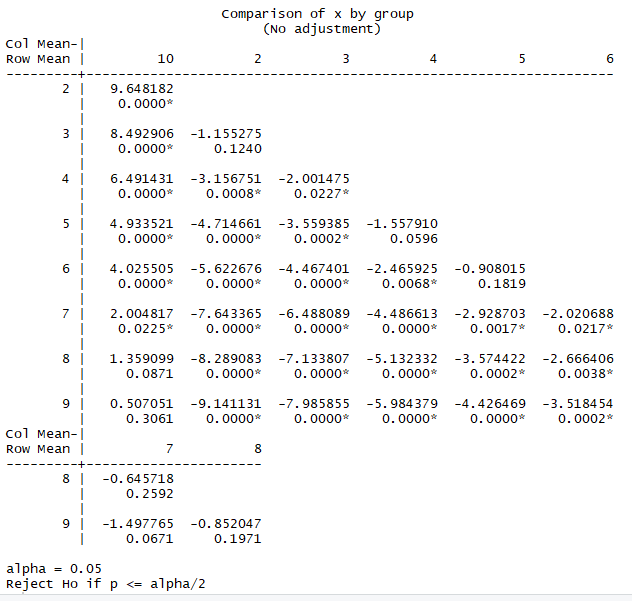
\includegraphics[width=9cm]{1.png} 
\caption{Porcentaje agentes infectados a traves del tiempo con pv = 0 y 0.1.}
\end{figure}
\begin{figure}[H]
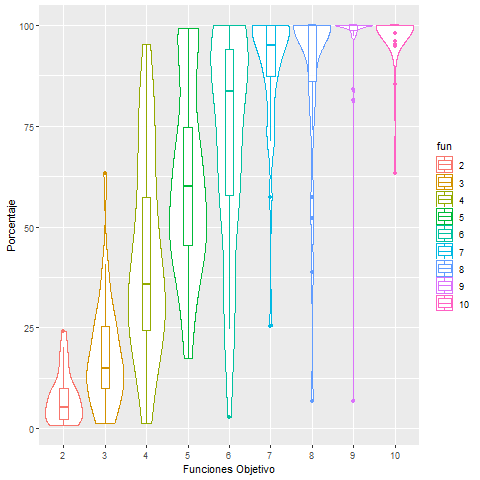
\includegraphics[width=9cm]{2.png}           \includegraphics[width=9cm]{3.png} 
\caption{Porcentaje agentes infectados a través del tiempo con pv = 0.2 y 0.3.}
\end{figure}
\begin{figure}[H]
\includegraphics[width=9cm]{4.png}           \includegraphics[width=9cm]{5.png} 
\caption{Porcentaje agentes infectados a través del tiempo con pv = 0.4 y 0.5.}
\end{figure}
\begin{figure}[H]
\includegraphics[width=9cm]{6.png}           \includegraphics[width=9cm]{7.png} 
\caption{Porcentaje agentes infectados a través del tiempo con pv = 0.6 y 0.7.}
\end{figure}
\begin{figure}[H]
\includegraphics[width=9cm]{8.png}           \includegraphics[width=9cm]{9.png} 
\caption{Porcentaje agentes infectados a través del tiempo con pv = 0.8 y 0.9.}
\end{figure}
En la Figura 6, se observa el comportamiento de la distribución de los agentes en cada iteración de pv usado. En la iteración 0.4 mostró un comportamiento más homogéneo entre los estados, en el cual la presencia de infección, susceptibilidad y recuperación de los agentes es muy similar, posteriormente le siguen las iteraciones de 0.6 y 0.3. 
\begin{figure}[H]
\centering
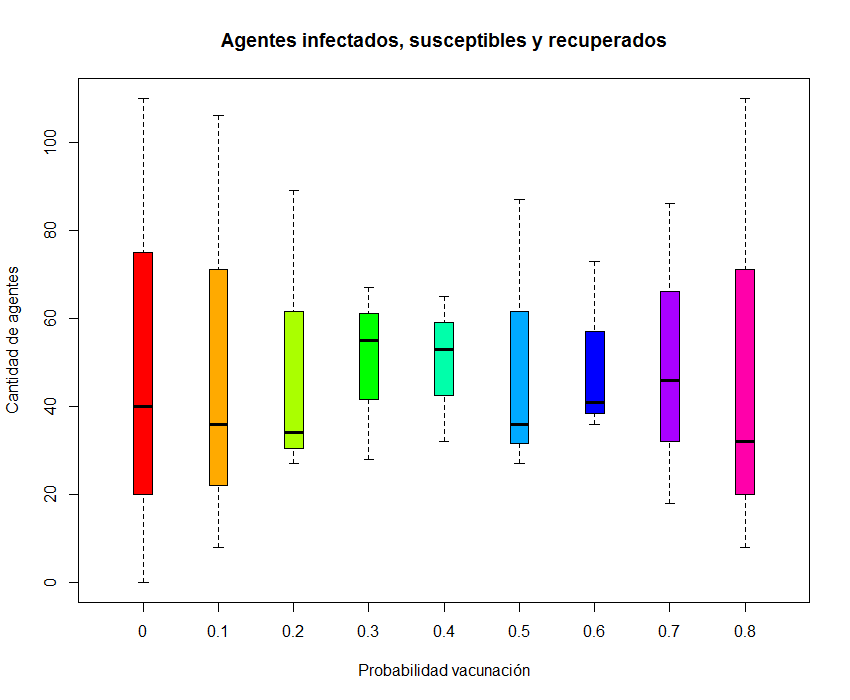
\includegraphics[width=13cm]{boxplot.png}
\caption{Comparación de la distribución de agentes con respecto a la probabilidad de estar vacunados, en donde se observa que la mejor distribución de la población se encuentra en el rango 0.4.}
\end{figure}
Además, en la Figura 6 se observa el cambio gradual que ocurre, principalmente en las 5 primeras iteraciones, y es en donde se comienza la redistribución del número de agentes en los diferentes estados y comienzan a colocarse en el estado R, esto se puede interpretar ya que los primeros resultados corresponden a una mayor cantidad de agentes infectados debido a que no había muchos vacunados, y esto se interpreta como una mayor distribución al estado I, el cual después de la iteración 0.4 se puede entender que cambia favoreciendo al del estado R. 

\section{Conclusiones}
La iteración que mostró una distribución más homogénea fue la de 0.4.
El comportamiento de la epidemia se mantuvo constante en las primeras 5 iteraciones, posterior a está su variación es mayor, como resultado la epidemia tiene casos en donde disminuye su frecuencia de aparición, sin embargo, está puede aumentar.


\bibliographystyle{plainnat}
\bibliography{ref6}




\end{document}